\documentclass[b0paper,margin=1cm,landscape]{baposter}

\usepackage{lipsum}          % This is just for some blindtext

\usepackage{relsize}	       % For \smaller
\usepackage{url}			       % For \url
\usepackage{epstopdf}	       % Included EPS files automatically converted to PDF to include with pdflatex
\usepackage{multicol}        % Multi Columns

\usepackage{amsmath,amssymb} % math
\usepackage{natbib}
\usepackage{graphicx}
\usepackage{xcolor}
 
\definecolor{umblue}{rgb}{0.03, 0.15, 0.30}
\definecolor{ummaize}{rgb}{0.90, 0.85 0.40}

%%%%%%%%%%%%%%%%%%%%%%%%%%%%%%%%%%%%%%%%%%%%%%%%%%%%%%%%%%%%%%%%%%%%%%%%%%%%%%%%
%%% Utility functions %%%%%%%%%%%%%%%%%%%%%%%%%%%%%%%%%%%%%%%%%%%%%%%%%%%%%%%%%%
%%%%%%%%%%%%%%%%%%%%%%%%%%%%%%%%%%%%%%%%%%%%%%%%%%%%%%%%%%%%%%%%%%%%%%%%%%%%%%%%

%%% Save space in lists. Use this after the opening of the list %%%%%%%%%%%%%%%%
\renewcommand{\vec}[1]{\bm{#1}}
\newcommand{\vnabla}{\vec{\nabla}}

\renewcommand{\d}[1]{\text{d} #1}
\newcommand{\dxx}{\,\text{d}\vec{x}}
\newcommand{\dx}{\,\text{d}x}

\newcommand{\diff}[2]{\frac{\text{d}#1}{\text{d}#2}}
\newcommand{\idiff}[2]{\text{d}#1 / \text{d}#2}
\newcommand{\pdiff}[2]{\frac{\partial #1}{\partial #2}}
\newcommand{\pdifff}[2]{\frac{\partial^2 #1}{\partial #2^2}}
\newcommand{\ipdiff}[2]{\partial #1 / \partial #2}
\newcommand{\vdiff}[2]{\frac{\delta #1}{\delta #2}}
\newcommand{\ivdiff}[2]{\delta #1 / \delta #2}

%%%%%%%%%%%%%%%%%%%%%%%%%%%%%%%%%%%%%%%%%%%%%%%%%%%%%%%%%%%%%%%%%%%%%%%%%%%%%%%
%%% Document Start %%%%%%%%%%%%%%%%%%%%%%%%%%%%%%%%%%%%%%%%%%%%%%%%%%%%%%%%%%%%
%%%%%%%%%%%%%%%%%%%%%%%%%%%%%%%%%%%%%%%%%%%%%%%%%%%%%%%%%%%%%%%%%%%%%%%%%%%%%%%

\begin{document}
\typeout{Poster rendering started}

%%% General Poster Settings %%%%%%%%%%%%%%%%%%%%%%%%%%%%%%%%%%%%%%%%%%%%%%%%%%%
%%%%%% Eye Catcher, Title, Authors and University Images %%%%%%%%%%%%%%%%%%%%%%
\begin{poster}{
  columns=3,
	grid=false,
	borderColor=umblue,
	headerColorOne=umblue,
	headerColorTwo=umblue,
	headerFontColor=ummaize,
  headerheight=11em,
	boxColorOne=white,
  boxpadding=1em,
	headershape=rectangle,
	headerfont=\Large\textsf,
	textborder=none,
	background=shadetb,
  bgColorOne=white,
  bgColorTwo=white,
	headerborder=open,
  boxshade=plain,
  headershade=plain,
  eyecatcher=false
}
%%% Eye Catcher %%%%%%%%%%%%%%%%%%%%%%%%%%%%%%%%%%%%%%%%%%%%%%%%%%%%%%%%%%%%%%%
{
}
%%% Title %%%%%%%%%%%%%%%%%%%%%%%%%%%%%%%%%%%%%%%%%%%%%%%%%%%%%%%%%%%%%%%%%%%%%
{Reinforcement Bias in Online Communities}
%%% Authors %%%%%%%%%%%%%%%%%%%%%%%%%%%%%%%%%%%%%%%%%%%%%%%%%%%%%%%%%%%%%%%%%%%
{
  \vspace{0mm}
  \textbf{Cason Konzer}

  \hspace{1mm} $ \downharpoonright $  \color{umblue}
  \textit{mailto:casonk@umich.edu} 
  \color{black}
  
  \hspace{1mm} $ \downharpoonright $ \color{umblue}
  \textit{https://github.com/casonk/pushshift\_python} 
  \color{black}
}
%%% Logo %%%%%%%%%%%%%%%%%%%%%%%%%%%%%%%%%%%%%%%%%%%%%%%%%%%%%%%%%%%%%%%%%%%%%%
{
  \begin{minipage}{9.0em}
    
\includegraphics[height=8em]{_img/University_of_Michigan_Flint.png}
  \end{minipage}
}

%%% Abstract %%%%%%%%%%%%%%%%%%%%%%%%%%%%%%%%%%%%%%%%%%%%%%%%%%%%%%%%%%%%%%%%%%
\headerbox{Abstract}{name=box00, column=0, row=0}{

  \hspace{5mm} Recent trends in information sharing have emphasized concerns of misinformation and the power of group activity. 
  A special attribute of online communities is their ability to grow rapidly. Similarly, information has been given the same attribute through the web. 
  As a culmination of these two factors, we have seen rapid manifestation of online phenomena in the real world. 
  Some recent examples of this phenomena are the widespread following of unknown political actor \textit{Q}, 
  retail trading frezny of \textit{meme stonks}, and the \textit{capital insurrection}. \\

  \hspace{5mm} Of particular intrest, is the development and group action of online comunities. 
  Well known is the ability to share and rate information exchange within online communities. 
  The following \textbf{research questions} have been developed to study the online information exchange \dots

  \textbf{
    \begin{enumerate}
      \item How do communal actors and entities direct users to recommended communities?
      \item Do communities with high bidirectional reference rates share similar audiences? content?
      \item Do communities with high bidirectional reference rates reinforce the ideas of one-another?
      Form an echochamber?
    \end{enumerate}
  }

  \hspace{5mm} In search of the answers to these questions, this project has focused on how communities reference one another.
  The platform of study is \textbf{Reddit}, due to the open sourced data provided by their public api and the public \textsl{PushShift.io} database.
  We study references defined through post embedded urls and posts containing tokens in the "r/<community>" form.
  We calculate Jaccard Similarity upon pairwise communities and inspect those pairs who have high bidirectional reference ratios.
  To gain additional insight, we calculate a Jaccard Similarity based on community autorship in the same pairwise manner.
  We believe communities of highest interest will exhibit high similarities in both co-refences and co-authors. 
  Continuing efforts are being made to categorize communities through text analysis metrics such as community subjectivity and polarity.
}

%%% Abstract %%%%%%%%%%%%%%%%%%%%%%%%%%%%%%%%%%%%%%%%%%%%%%%%%%%%%%%%%%%%%%%%%%
\headerbox{Reference Extraction}{name=box01, column=0, row=1, above=bottom, below=box00}{

  \hspace{5mm} To illustrate what we define as a reference, consider two examples. 
  We will assume both of these examples are based in the Reddit r/Database community.  
  \begin{enumerate}
    \item post with embedded url: \url{http://www.reddit.com/r/SQL/}
    \item post with body: \texttt{Visit our friends over at r/SQL and /Oracle.}
  \end{enumerate}

  \hspace{5mm} In both of the posts, we extract SQL as a referenced community and save as a directional pair, r/Database $ \longmapsto $ r/SQL.
  To minimize false positives, the destination community is cross-referenced with a compiled set of all communities. 
  As a result, the reference is only saved given, SQL $ \in $ All-Subreddits.
  Where the reference metric lacks is in the false negative space. 
  As seen in example 2, references can easily be missed due to lack of prefix.
  To capture the references such as r/SQL, we perform splits on "r/" and then extract the trailing string.
  Altough, due to spelling errors, there is still chance for false negatives granted our expected prefix.
  One attempt to capture unprefixed references such as /Oracle is through a bag of words approach. 
  In a similar fashion as before, we can split the post text into tokens and check if each token is in our set of subreddits.
  Additional challenges follow as a community name may be uses without reference. For example, "The Oracle down the road has recommended I take up logic."
  Further developement is to come and suggestions are welcomed. 

}

%%% Graphics %%%%%%%%%%%%%%%%%%%%%%%%%%%%%%%%%%%%%%%%%%%%%%%%%%%%%%%%%%%%%%%%%%
\headerbox{Figures 1,2,3,4}{name=box10, column=1, row=0}{

    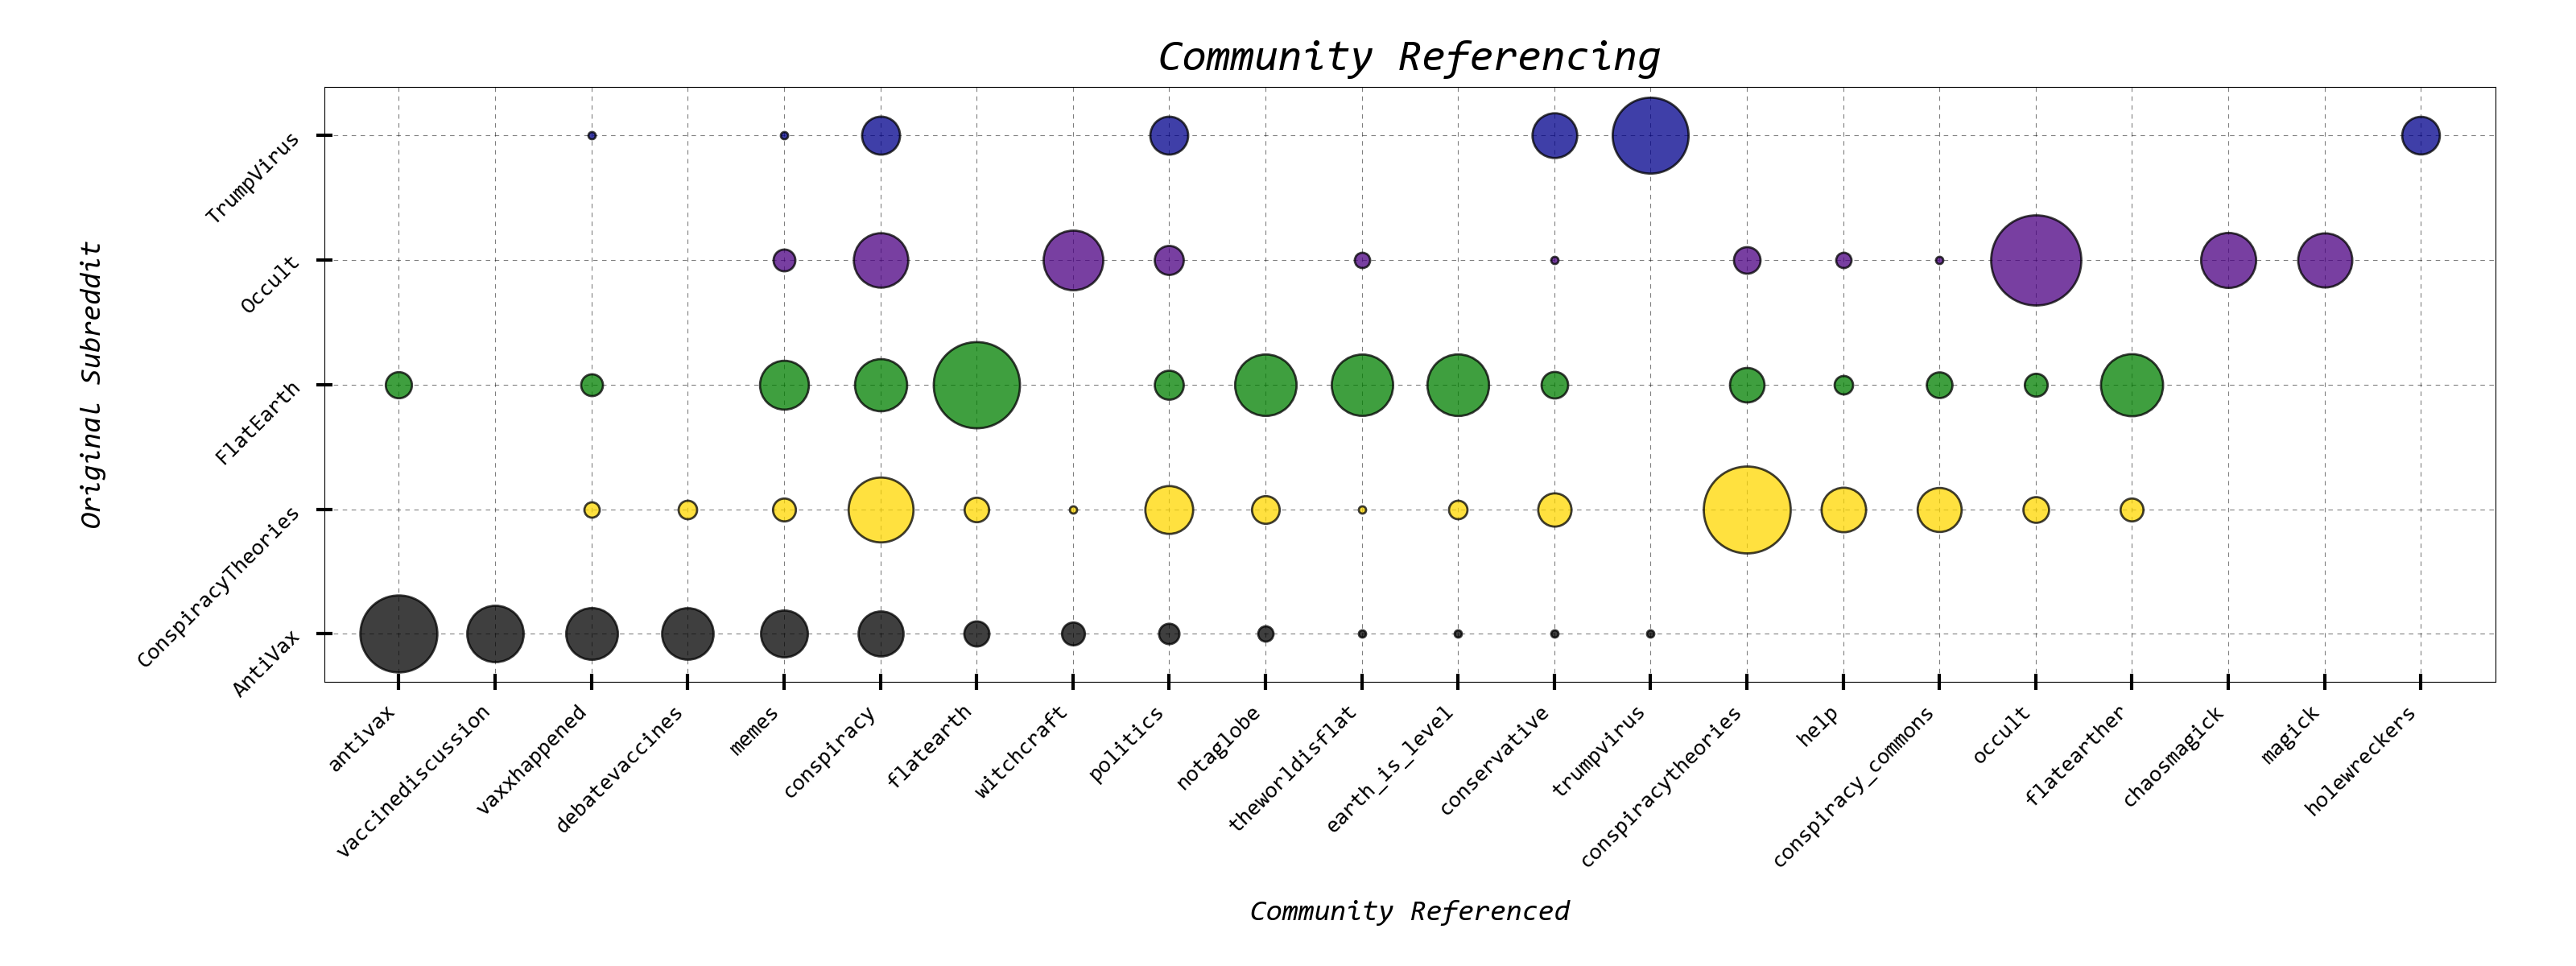
\includegraphics[width=.901\textwidth]{_img/References.png}

    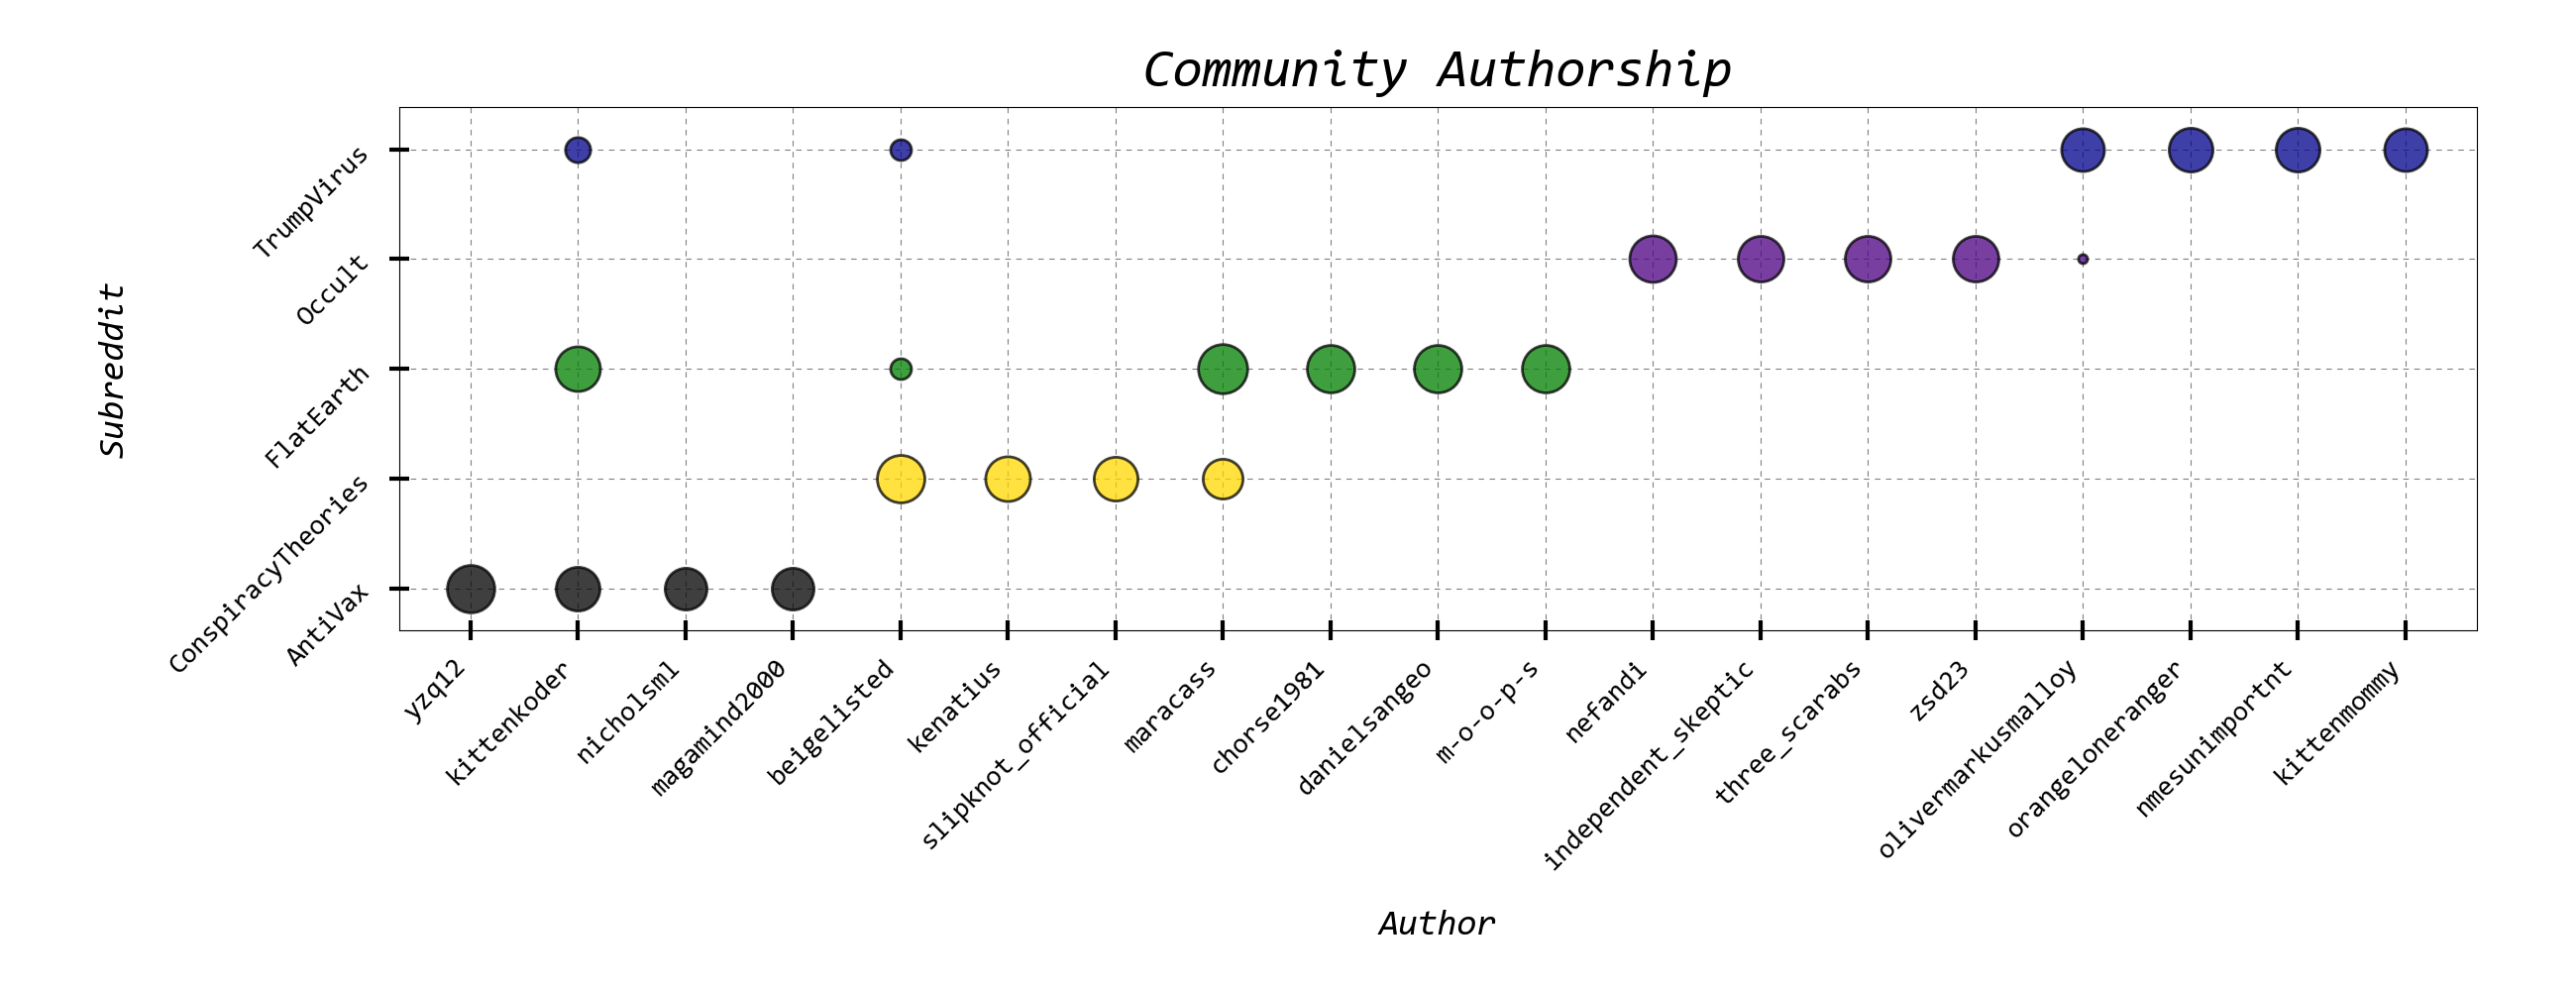
\includegraphics[width=.901\textwidth]{_img/Authors.png}

    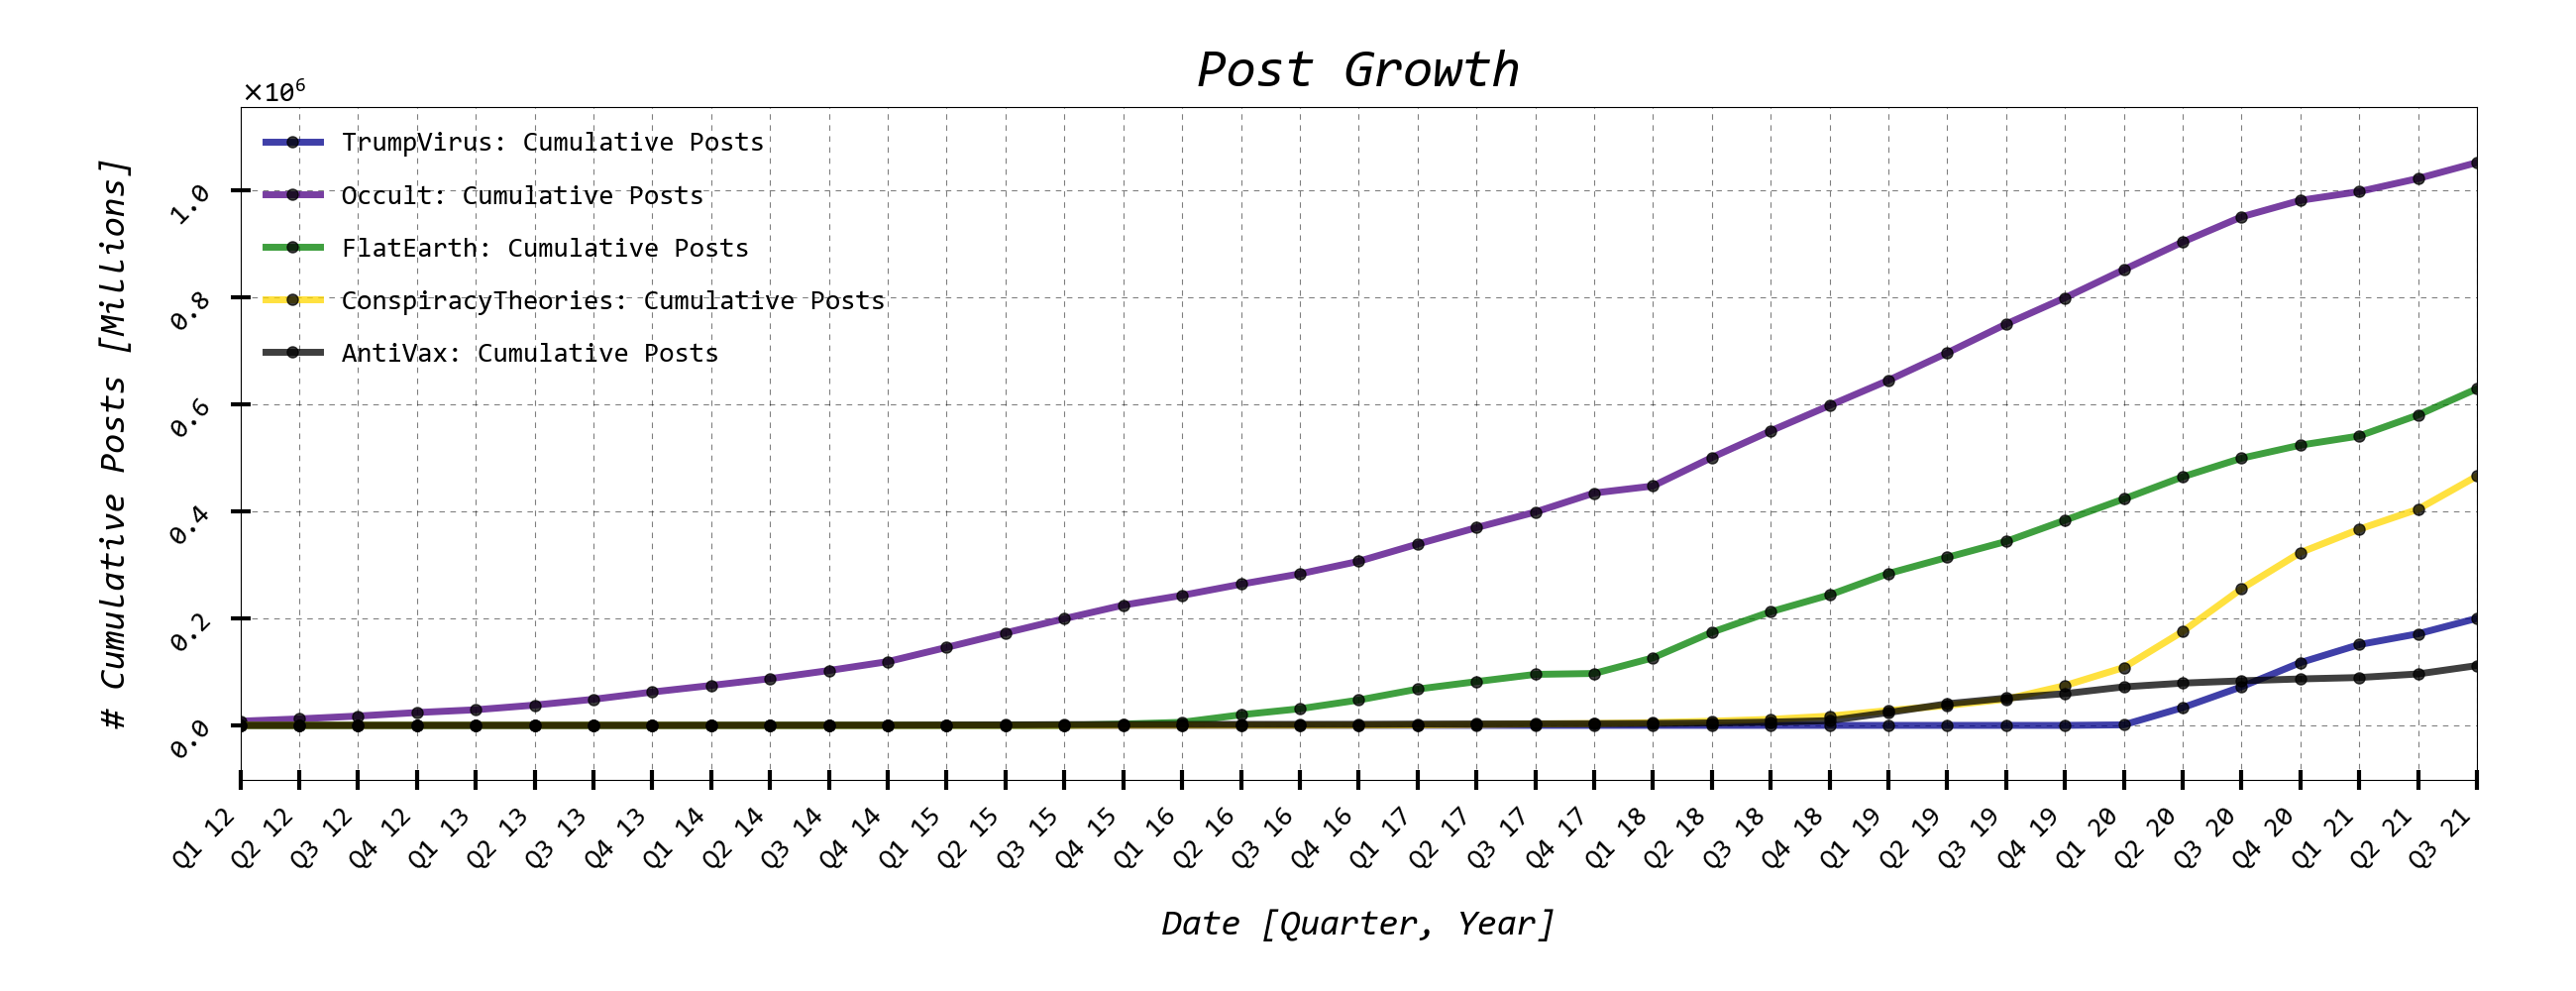
\includegraphics[width=.901\textwidth]{_img/growth.png}

  \begin{center}
    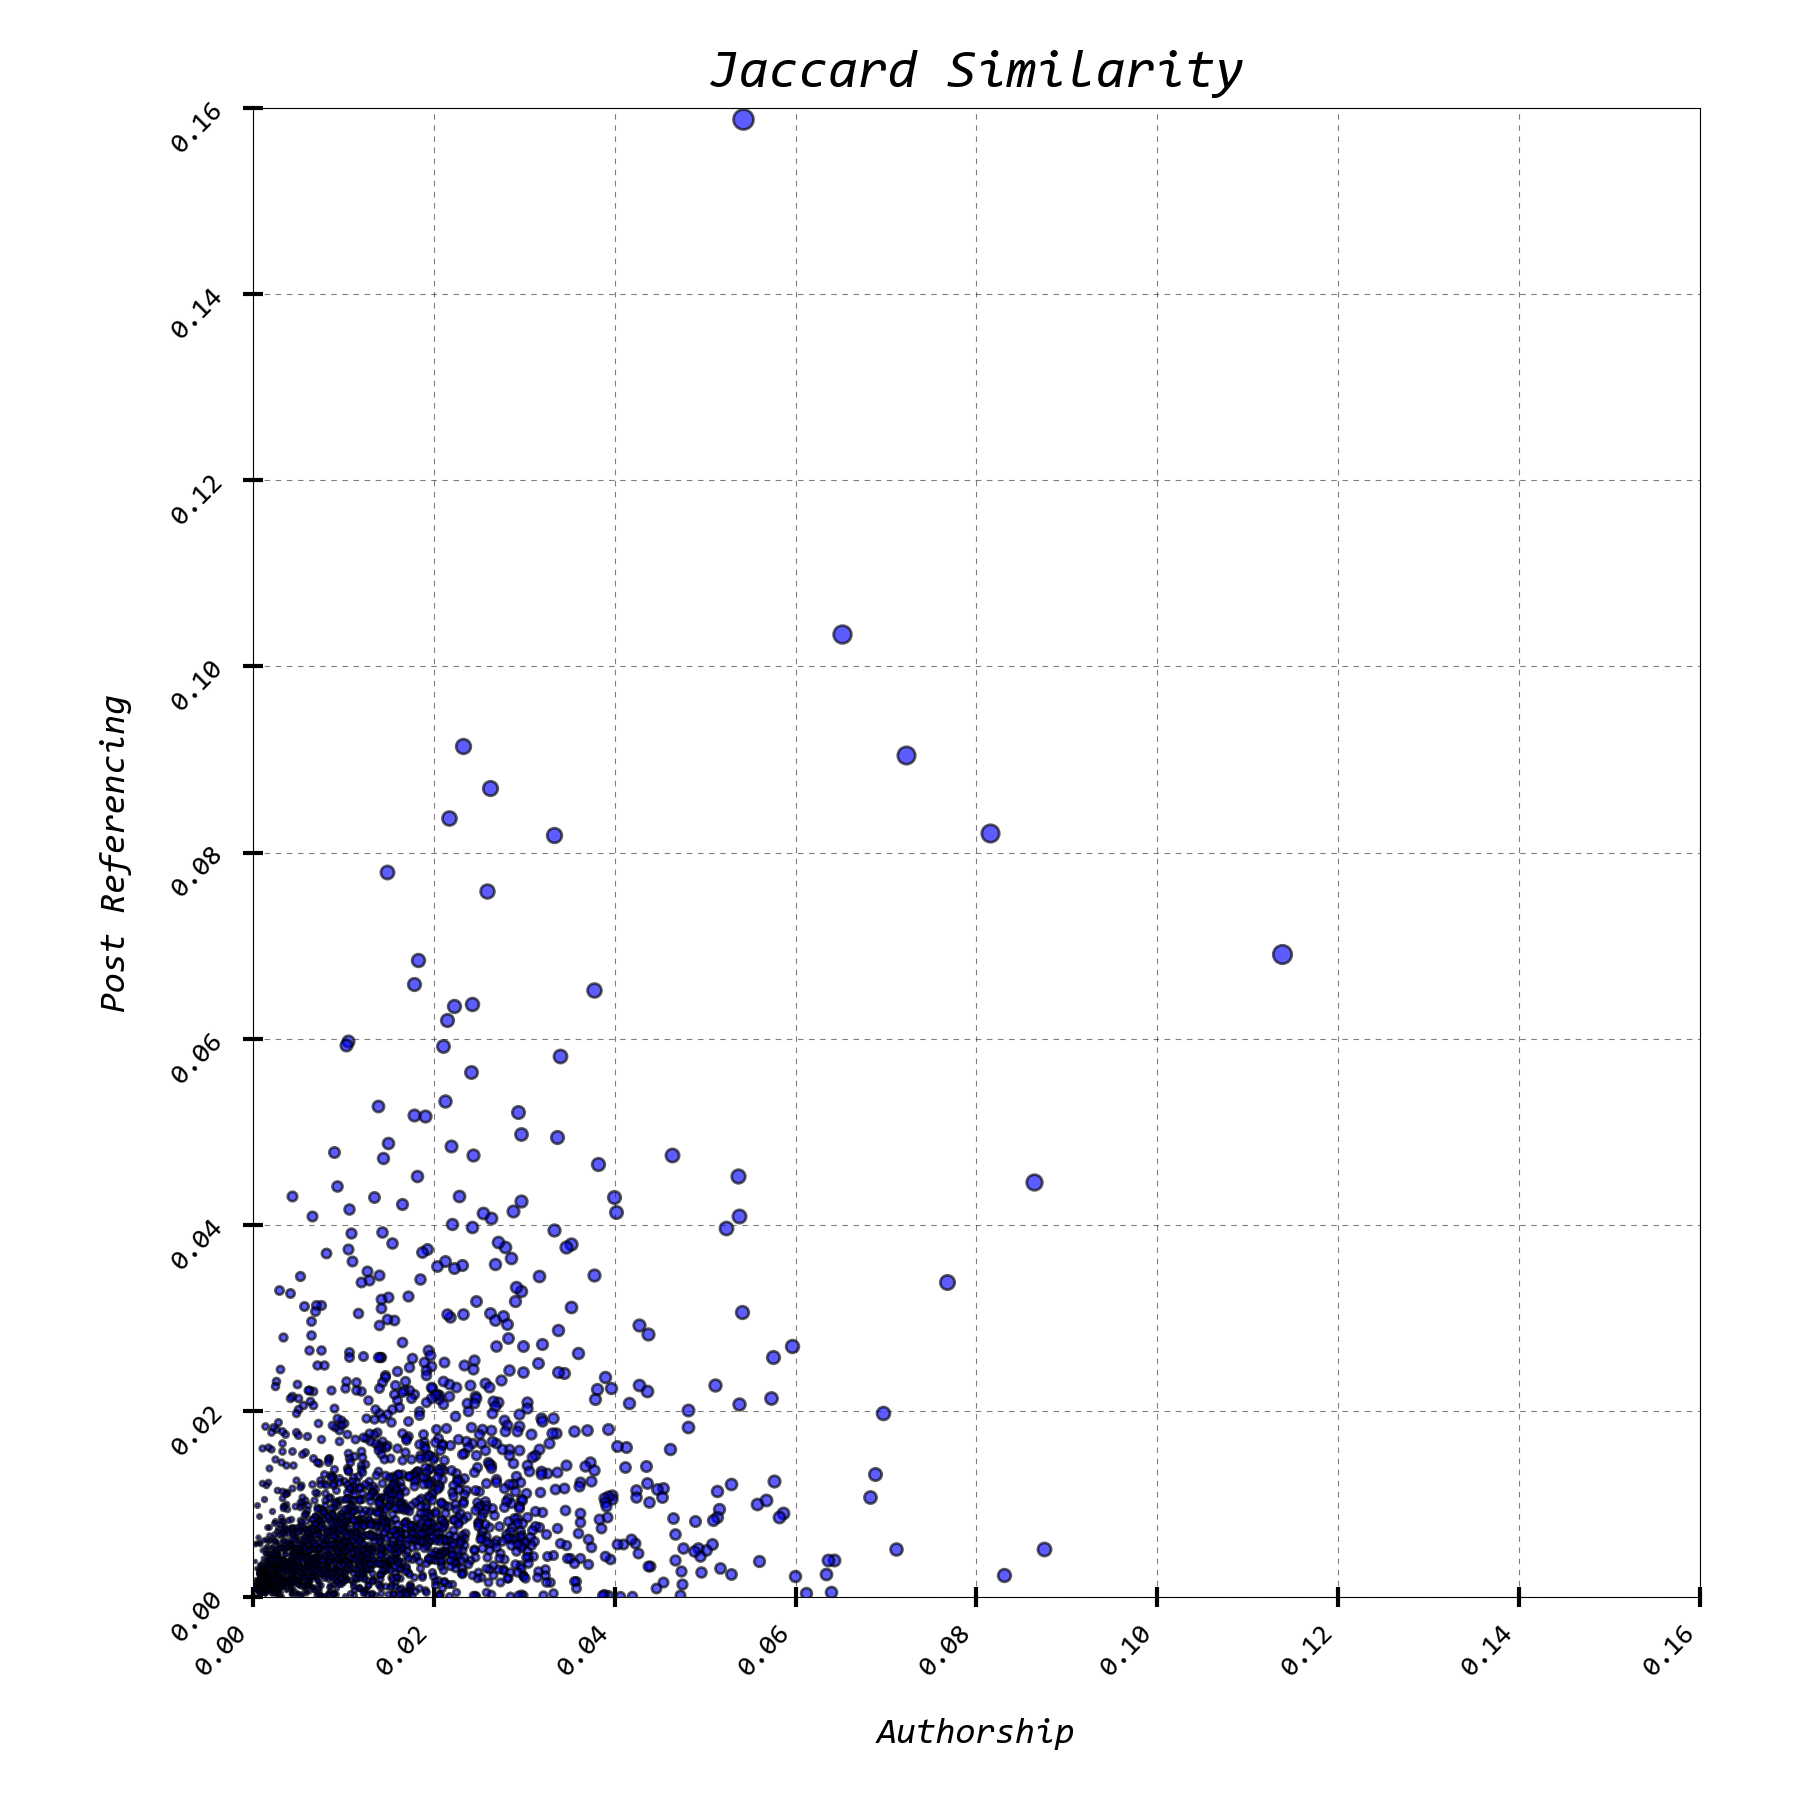
\includegraphics[width=.731\textwidth]{_img/Jaccard_Similarity.png}
  \end{center}

  \textsl{Figures Labeled as Top to Bottom 1-4}

}


%%% Descriptions %%%%%%%%%%%%%%%%%%%%%%%%%%%%%%%%%%%%%%%%%%%%%%%%%%%%%%%%%%%%%%%%%%%%%
\headerbox{Figure Descriptions}{name=box20, column=2, row=0}{

  \hspace{5mm}
  \textsl{\underline{Note}: For the following charts, we use an arbitrarily chosen set of origin communities to study.
  In future research we seek to use a larger set and then select those communities displaying emergent features.}

  
  \begin{enumerate}

    \vspace{1.5mm}
    \item \textsl{\textbf{Community Referencing:}}
    \subitem In this figure, each node represents a pairwise relationship, origin $ \longmapsto $ destination community $\langle y$-$axis \longmapsto x$-$axis \rangle$.
    Each node on the graph is weighted by the number of directional occurences. 
    An emerging factor is that the self reference appears most frequent, origin $ \longmapsto $ origin.
    Node selection is based on the top 5 references from each origin communitiy. 
    Due to overlap within the sets of top references, the sum referenced communities displayed is only 22, despite having 5 communities. 
    
    \vspace{1em}
    \item \textsl{\textbf{Community Authorship:}}
    \subitem The structure is similar within this chart as well, although the results are much different. 
    Here the $y$-$axis$ represents the origin community as before, and the $ x $-$ axis $ represents the top 5 authors for these communities.
    As a note, we blacklist 3 of the most common author names: \textit{[deleted], automoderator, and sneakpeekbot}.
    What is interesting from the chart is that overlap is much less present than seen above. The top authors of the communities are more isolated. 
    
    \vspace{1em}
    \item \textsl{\textbf{Post Growth:}}
    \subitem Two additional metrics to factor are community growth rates and time since inception. 
    By plotting multiple communities, trends become more evident and provide a means for comparison. 
    Here the $y$-$axis$ represents the number of posts made within the community(in millions). 
    We define a post as either an original submission or a comment on such submissions. 
    Each $x$-$tick$ represents a quarter, or 4 months, following the time scale the axis represents. 
    Important is that each successive quarter adds the posts realized to the previous quarter.
    
    \vspace{1em}
    \item \textsl{\textbf{Jaccard Similarity:}}
    \subitem This final plot builds upon figure 1 and figure 2. 
    Jaccard Similarity is used as a measure of overlap and is defined as $ \mathcal{J} $.
    We use $C_i$ to denote a community of interest. 
    To solve for the the authorship similarity, we have $ \mathcal{J}_a $.
    In calculating both the authorship and reference similarities, we look at the pairs within each community for a given author $ a $ or reference $ r $.
    If an author posts 10 times in communitiy $ 1 $ and 5 times in community $ 2 $, we have $ min (\# C_{1_a}, \# C_{2_a}) = $ 5 and $ (\# C_{1_a} + \# C_{2_a}) =$ 15.
    The solution follows with references, such that a reference is made 10 and 5 times in communities $ 1 $ and $ 2 $.
    We do this for each author and reference within the sets $ A $ and $ R $, encompassing the union of all authors posting or references made in either community $1$ or $2$.
    If an author never posts, or a reference is never made, in one of the two communities, it is given a score of 0 for that community. 
    We then plot $ \mathcal{J}_a X \mathcal{J}_r $ on the graph and repeat for each pairwise community within the set of communities we have data collected on. 
    We start with 69 communities and plot 2,346 total pairs. 
    From our set, we can see the majority of communities are not similar. 
    Future research entails analysis on a larger set of highly active communities. 
    \begin{center}
      $ \displaystyle \mathcal{J} = \frac{\vert C_1 \cap C_2 \vert }{\vert C_1 \cup C_2 \vert } $. \vspace{10mm}
      $ \displaystyle \mathcal{J}_{a,r} = \frac{\sum_{a,r}^{A,R} \ min (\# C_{1_{a,r}}, \# C_{2_{a,r}})}{\sum_{a,r}^{A,R} \ (\# C_{1_{a,r}} + \# C_{2_{a,r}}) - \sum_{a,r}^{A,R} \ min (\# C_{1_{a,r}}, \# C_{2_{a,r}})} $. \vspace{10mm}
    \end{center}

  \end{enumerate}

}

\end{poster}
\end{document}
